\documentclass[11pt,letterpaper, leqno]{article}
\usepackage{latexsym}
\usepackage{amsmath}
\usepackage{amssymb}
\usepackage{amsthm}
\topmargin -0.25in
\textheight 8.5in
\oddsidemargin 0.0in
\textwidth 6.5in

\RequirePackage{amsthm,amsmath,amsfonts,amssymb}
%\RequirePackage[numbers]{natbib}
\RequirePackage[authoryear]{natbib}%% uncomment this for author-year citations
\RequirePackage[colorlinks,citecolor=blue,urlcolor=blue]{hyperref}%% uncomment this for coloring bibliography citations and linked URLs
\RequirePackage{graphicx}%% uncomment this for including figures

\usepackage{tikz}
\usepackage{graphicx}
\usepackage{natbib}
\usepackage{authblk}
\usepackage{enumerate}
\usepackage{bbm}

\usepackage{listings}
\usepackage{xcolor}
\usepackage{fancyhdr}

\definecolor{codegreen}{rgb}{0,0.6,0}
\definecolor{codegray}{rgb}{0.5,0.5,0.5}
\definecolor{codepurple}{rgb}{0.58,0,0.82}
\definecolor{backcolour}{rgb}{0.95,0.95,0.92}

\lstdefinestyle{mystyle}{
    backgroundcolor=\color{backcolour},   
    commentstyle=\color{codegreen},
    keywordstyle=\color{magenta},
    numberstyle=\tiny\color{codegray},
    stringstyle=\color{codepurple},
    basicstyle=\ttfamily\footnotesize,
    breakatwhitespace=false,         
    breaklines=true,                 
    captionpos=b,                    
    keepspaces=true,                 
    numbers=left,                    
    numbersep=5pt,                  
    showspaces=false,                
    showstringspaces=false,
    showtabs=false,                  
    tabsize=2
}

\lstset{style=mystyle}

\usepackage[english]{babel}
\bibliographystyle{abbrvnat}
\setcitestyle{authoryear,open={(},close={)}}

% For the algorithm table
\usepackage{algorithm,algcompatible,amsmath}
\DeclareMathOperator*{\argmax}{\arg\!\max}
\DeclareMathOperator*{\argmin}{\arg\!\min}
% https://tex.stackexchange.com/q/83169/5764
\algnewcommand\INPUT{\item[\textbf{Input:}]}%
\algnewcommand\OUTPUT{\item[\textbf{Output:}]}%
%

% the settings of tikz is used for the optimization of the graphs  
\usetikzlibrary{shapes, arrows, calc, arrows.meta, fit, positioning} % these are the parameters passed to the library to create the node graphs  
\tikzset{  
    -Latex,auto,node distance =1.5 cm and 1.3 cm, thick,% node distance is the distance between one node to other, where 1.5cm is the length of the edge between the nodes  
    state/.style ={ellipse, draw, minimum width = 0.9 cm}, % the minimum width is the width of the ellipse, which is the size of the shape of vertex in the node graph  
    point/.style = {circle, draw, inner sep=0.18cm, fill, node contents={}},  
    bidirected/.style={Latex-Latex,dashed}, % it is the edge having two directions  
    el/.style = {inner sep=2.5pt, align=right, sloped}  
}  


\newtheorem{theorem}{Theorem}
\newtheorem{acknowledgement}[theorem]{Acknowledgement}
%\newtheorem{algorithm}[theorem]{Algorithm}
\newtheorem{axiom}[theorem]{Axiom}
\newtheorem{problem}[theorem]{Problem}
\newtheorem{remark}{Remark}
\newtheorem{claim}[theorem]{Claim}
\newtheorem{conclusion}[theorem]{Conclusion}
\newtheorem{condition}[theorem]{Condition}
\newtheorem{conjecture}[theorem]{Conjecture}
\newtheorem{corollary}{Corollary}
\newtheorem{criterion}[theorem]{Criterion}
\newtheorem{definition}{Definition}
\newtheorem{example}{Example}
\newtheorem{exercise}[theorem]{Exercise}
\newtheorem{lemma}{Lemma}
\newtheorem{proposition}{Proposition}
\newtheorem{thm}{Theorem}[section]
\newtheorem{lem}{Lemma}[section]
\newtheorem{prop}{Proposition}[section]
\newtheorem{defn}{Definition}[section]
\newtheorem{ex}{Example}[section]
\newtheorem{cor}{Corollary}[section]
\newtheorem{rem}{Remark}[section]
\newtheorem{rems}{Remarks}[section]
\numberwithin{equation}{section} 
\numberwithin{theorem}{section}
\numberwithin{lemma}{section} 
\numberwithin{corollary}{section}
\numberwithin{definition}{section}
\numberwithin{proposition}{section} 
\numberwithin{remark}{section}
\numberwithin{example}{section}
\newtheorem{assumption}{Assumption}
\DeclareMathOperator\supp{supp}

%\newcommand{\ex}{{\bf\sf E}}            %% expectation
\newcommand{\bfp}{{\bf P}}
\newcommand{\bfr}{{\bf R}}
\newcommand{\Var}{{\rm Var}}            %% 
\newcommand{\Cov}{{\rm Cov}}            %% 
\newcommand{\calc}{{\cal C}}            %%
\newcommand{\cald}{{\cal D}} 
\newcommand{\calf}{{\cal F}}            %%
\newcommand{\call}{{\cal L}}            
\newcommand{\al}{\alpha}                %%
\newcommand{\bt}{\beta}                %%
\newcommand{\ga}{\gamma}                %% abbreviated
\newcommand{\dt}{\delta}                %% greek letters
\newcommand{\la}{\lambda}               %%
\newcommand{\ep}{\epsilon}              %%
\newcommand{\sig}{\sigma}               %%
\newcommand{\tri}{\triangle}
\newcommand{\om}{\omega}                %%
\newcommand{\ra}{\rightarrow}           %%
\newcommand{\lra}{\longrightarrow}
\newcommand{\Ra}{\Rightarrow}           %% arrows
\newcommand{\subs}{\subseteq}           %% subset or equal to
\newcommand{\eqdef}{\stackrel{\triangle}{=}}
\newcommand{\hY}{\hat{Y}}
\newcommand{\hp}{\hat{p}}
\newcommand{\hX}{\hat{X}}
\newcommand{\hy}{\hat{y}}
\newcommand{\hQ}{\hat{Q}}
\newcommand{\Zh}{\hat{Z}}
\newcommand{\hla}{\hat{\lambda}}
\newcommand{\starti}{\parindent0pt\it}  %% start an italic line
\newcommand{\startb}{\parindent0pt\bf}  %% start a boldface line
\newcommand{\tril}{\triangle^-}
\newcommand{\trir}{\triangle^+}
\newcommand{\trilr}{\triangle^{\pm}}
\newcommand{\realR}{{{\rm I}\;\!\!\!{\rm R}}}
\newcommand{\probP}{{{\rm I}\;\!\!\!{\rm P}}}
\newcommand{\filtF}{{{\rm I}\;\!\!\!{\rm F}}}
\newcommand{\expeE}{{{\rm I}\;\!\!\!{\rm E}}}
\newcommand{\noin}{{\noindent}}
\newcommand{\doty}{{\dot{y}}}
\newcommand{\doth}{{\dot{h}}}
\newcommand{\dotx}{{\dot{x}}}
\newcommand{\dotu}{{\dot{u}}}
\newcommand{\dotf}{{\dot{f}}}
\newcommand{\dotg}{{\dot{g}}}
\newcommand{\ddoty}{{\ddot{y}}}
\newcommand{\ddoth}{{\ddot{h}}}
\newcommand{\ddotx}{{\ddot{x}}}
\newcommand{\ddotf}{{\ddot{f}}}
%\newcommand{\Var}{{\mbox{Var}}}
%\newcommand{\Cov}{{\mbox{Cov}}}
\newcommand{\T}{\intercal}

\renewcommand{\Var}{\text{Var}}
\renewcommand{\P}{\mathbb{P}}
\newcommand{\R}{\mathbb{R}}
\newcommand{\E}{\mathbb{E}}
\newcommand{\Z}{\mathbb{Z}}
\renewcommand{\qed}{\quad \blacksquare}
\newcommand{\ind}{\mathbbm{1}}

\begin{document}
\begin{center}
{\bf \Large APMA1690: ~~Homework \# 2 ~~~(Due by 11pm Sep 28)}
\end{center}
\[\]
\medskip

\section{Question 1}\label{Question 1}

\subsection{Review before Question \ref{Question 1}: the Law of Large Numbers (LLN)}

\begin{theorem}[Etemadi's strong LLN, 1981, see \cite{etemadi1981elementary} or Theorem 5.17 of \cite{klenke2013probability}]\label{thm: Etemadi's strong LLN}
Let $Z_1, Z_2, \ldots$ be real-valued random variables defined on probability space $(\Omega,\mathbb{P})$. Suppose they are identically distributed and \href{https://en.wikipedia.org/wiki/Pairwise_independence}{pairwise independent} (i.e., $Z_i$ and $Z_j$ are independent for all $i,j$ with $i\ne j$). If $\mathbb{E} Z_1$ exists, then $\lim_{n\rightarrow\infty}\left(\frac{1}{n}\sum_{i=1}^nZ_i\right)=\mathbb{E}Z_1$ with probability one, i.e.,
\begin{align}\label{eq: Etemadi's strong LLN}
    \mathbb{P}\left\{\omega\in\Omega: \lim_{n\rightarrow\infty}\left(\frac{1}{n}\sum_{i=1}^n Z_i(\omega)\right)=\mathbb{E}Z_1\right\}=1.
\end{align}
\end{theorem}


\subsection{Setup of Question \ref{Question 1}}

Let $(\Omega,\mathbb{P})$ be a probability space as follows
\begin{itemize}
    \item The set $\Omega$ is defined by
    \begin{align*}
        \Omega= \underbrace{\{0,1\} \times \{0,1\} \times \cdots \times \{0,1\} \times \cdots}_{\mbox{\href{https://en.wikipedia.org/wiki/Cartesian_product}{Cartesian product}, infinitely many }\{0,1\}},
    \end{align*}
    where each element $\omega\in\Omega$ is an infinitely long vector of the form $\omega=\underbrace{(\omega_1, \omega_2,\ldots,\omega_n,\ldots)}_{\mbox{infinitely many entries}}$, and $\omega_i\in\{0,1\}$ for any positive integer $i$.
    \item $\mathbb{P}$ is a probability and satisfies the following: for any positive integer $i$, we have
    \begin{align*}
        \mathbb{P}\left\{\omega=(\omega_1, \omega_2,\ldots,\omega_n,\ldots)\in\Omega \,\vert\, \omega_i=1\right\} = \mathbb{P}\left\{\omega=(\omega_1, \omega_2,\ldots,\omega_n,\ldots)\in\Omega \,\vert\, \omega_i=0\right\} = \frac{1}{2};
    \end{align*}
    furthermore, for any positive integer $k$ and any vector
    \begin{align*}
        \boldsymbol{v}=(v_1,v_2,\ldots,v_k)\in \underbrace{\{0,1\}\times\cdots\times\{0,1\}}_{\mbox{\href{https://en.wikipedia.org/wiki/Cartesian_product}{Cartesian product}, $k$ times}},
    \end{align*}
    we have $\mathbb{P}\left\{\omega=(\omega_1, \omega_2,\ldots,\omega_n,\ldots)\in\Omega \,\vert\, \omega_i=v_i \mbox{ for all }i=1,2,\ldots,k\right\}=(1/2)^k$.
\end{itemize}
We define the following two subsets of $\Omega$
\begin{align*}
    & \Omega_1=\left\{\omega=(\omega_1, \omega_2,\ldots,\omega_n,\ldots)\in\Omega \,\Bigg\vert\, \lim_{n\rightarrow\infty}\left[\frac{1}{n}\sum_{i=1}^n \omega_i\right]=\frac{1}{2}\right\}, \\
    & \Omega_0=\left\{\omega=(\omega_1, \omega_2,\ldots,\omega_n,\ldots)\in\Omega \,\Bigg\vert\, \lim_{n\rightarrow\infty}\left[\frac{1}{n}\sum_{i=1}^n \omega_i\right] \ne \frac{1}{2}\right\};
\end{align*}

\subsection{Question \ref{Question 1}}

\begin{enumerate}[a]
    \item \textcolor{purple}{(1 points) For the following two elements $\omega^{(1)}$ and $\omega^{(2)}$ in $\Omega$, which of them belongs to $\Omega_1$? Which of them belongs to $\Omega_0$? Explain (rather than mathematically prove) your answer.
    \begin{align*}
        & \omega^{(1)}=(1,0,0,1,0,0,1,0,0, \ldots),\ \ \ \ \mbox{ (repetition of the ``1,0,0" pattern)},\\
        & \omega^{(2)}=(1,0,1,0,1,0,1,0,\ldots),\ \ \ \ \mbox{ (repetition of the ``1,0,1,0" pattern)}.
    \end{align*}}

    \color{blue}
        Both elements are members of $\Omega_1$. By the law of large numbers, the average should tend towards the expected value which is $1/2$ because having a $1$ or a $0$ is equally likely at each index.
    \color{black}

    \item \textcolor{purple}{(2 points) Prove the following using the LLN in a rigorous way
    \begin{align*}
        \mathbb{P}(\Omega_1)=1 \ \ \mbox{ and }\ \ \ \mathbb{P}(\Omega_0)=0.
    \end{align*}}

    \color{blue}
        Let $\{X_i\}_{i=1}^\infty$ be an infinite sequence of iid random variables such that $X_1 \sim \text{Bernoulli}(\frac{1}{2})$. Then 
        \[\E X_1 = 0\cdot \P(X = 0) 1\cdot \P(X = 1) = \P(X = 1) = \frac{1}{2}\]
        and
        \begin{align*}
            \P(\Omega_1) &= \P\left(\{\vec{\omega} \in \Omega \bigg\vert \;\lim_{n\to \infty} \left[\frac{1}{n}\sum_{i=0}^n X_i\right]  = \frac{1}{2}\}\right)\\
            &= \P\left(\{\vec{\omega} \in \Omega \bigg\vert \; \lim_{n\to \infty} \left[\frac{1}{n}\sum_{i=0}^n X_i\right] = \E X_1 \}\right)\\
            &\overset{LLN}{=} 1
        \end{align*}

        Then because $\Omega_1$ and $\Omega_0$ partition $\Omega$, we know that 
        \[\P(\Omega) = \P(\Omega_1) + \P(\Omega_0) \implies 1 = 1 + \P(\Omega_0) \implies \P(\Omega_0) = 0 \quad \blacksquare\]
    \color{black}
\end{enumerate}
\pagebreak

\section{Question 2}\label{Q2}

\subsection{Review before Question \ref{Q2}}

We have the following two versions of the \href{https://en.wikipedia.org/wiki/Law_of_the_iterated_logarithm}{Law of the Iterated Logarithm}
\begin{itemize}
    \item (Heuristic/sloppy version.) Suppose $X_1,\ldots,X_n,\ldots$ are iid random variables defined on the probability space $(\Omega, \mathbb{P})$. The mean is $\mu=\mathbb{E}X_1$ and the standard deviation is $\sigma=\sqrt{Var(X_1)}$. Then, we ``approximately" (rather than ``exactly") have the following inequality when the sample size $n$ is very large, where ``$\log$" is the \href{https://en.wikipedia.org/wiki/Natural_logarithm}{natural logarithm}.
    \begin{align*}
        \left\vert\frac{1}{n}\sum_{i=1}^n X_i(\omega)-\mu\right\vert \le \sigma\cdot\sqrt{\frac{2\cdot\log\left(\log n\right)}{n}}.
    \end{align*}
    \item (Mathematical/rigorous version, see Theorem 22.11 of \cite{klenke2013probability}; not required) Suppose $X_1,\ldots,X_n,\ldots$ are iid random variables defined on the probability space $(\Omega, \mathbb{P})$. The mean is $\mu=\mathbb{E}X_1$ and the standard variance is $\sigma=\sqrt{Var(X_1)}$. Then, we have
    \begin{align*}
    \mathbb{P}\left\{\omega\in\Omega \,\Bigg\vert \, \limsup_{n\rightarrow\infty}\left[\frac{\left\vert\frac{1}{n}\sum_{i=1}^n X_i(\omega)-\mu\right\vert}{\sigma\cdot\sqrt{\frac{2\cdot\log\left(\log n\right)}{n}}}\right]=1\right\}=1.
\end{align*}
\end{itemize}

\subsection{Question \ref{Q2}}

Use any programming language of your choice to execute the following steps:\\
Step 1: Generate 10,000 random numbers \(x_1, x_2, \ldots , x_{10000}\) from the distribution \(\operatorname{Bernoulli}(0.5)\). \\
Step 2: For each \(n\) in the range 100 to 10,000, compute \(y_n\) using the formula $y_n = \left| \frac{1}{n} \sum_{i=1}^n x_i - 0.5 \right|$. \\
Step 3: Plot the graph of ``\(y_n\) versus \(n\)" (with \(n\) on the horizontal axis). \\
Step 4: Repeat Steps 1-3 nine more times, and overlay all ten graphs on the same plot. \\
Step 5: Define a function $g(n) = 0.5 \cdot \sqrt{\frac{2 \cdot \log(\log n)}{n}}$. Then, add the graph of ``\(g(n)\) versus \(n\)" to the plot from Step 4. 

\textcolor{purple}{Display the picture obtained in Step 5 and provide the code used to generate it (2 points). Explain the picture from Step 5 (1 point).}

\includegraphics*[width=0.7\textwidth]{Images/q2.png}
\color{blue}
    \begin{verbatim}
        import matplotlib.pyplot as plt
        from scipy.stats import bernoulli
        from math import sqrt, log

        def avg(lst):
            return sum(lst)/len(lst)

        len_rands = 10000
        x = range(100, len_rands)

        for plot in range(10):
            rands = bernoulli.rvs(0.5, size=len_rands)
            running_avg = 0
            y = []
            for n in x:
                running_avg = ((running_avg * (n-1)) + (rands[n] - 0.5))/n
                y.append(abs(running_avg))
            plt.plot(x, y)

        g = list(map(lambda n: 0.5 * sqrt((2 * log(log(n)))/n), x))
        plt.plot(x, g, label="g(n)")

        plt.xlabel("n")
        plt.ylabel("y")
        plt.legend()
        plt.show()
    \end{verbatim}

    The plot shown above illustrates the law of the iterated logarithm. First, I generated a series of iid random variables $\{X_i\}_{i = 1}^{10000} \sim \text{Bernoulli}\left(\frac{1}{2}\right)$ with $\mu = \E X_1 = \frac{1}{2}$. Then for larger and larger $n$, I plotted the mean absolute error 
    \[e_n = |\overline X - \mu|\]
    for ten different series of random variables to illustrate that they all share a similar shape but are random. Finally, the function $g(n)$ is the quantity $\sqrt{\Var X_1} \cdot \sqrt{\frac{2\log\log n}{n}}$. The final graph confirms the heuristic that the running error is less than the quantity $g(n)$.
\color{black}
\pagebreak

\section{Question 3}\label{Q3}

\subsection{Review before Question \ref{Q3}}

\begin{itemize}
    \item (Empirical CDF.) Let $X_1, X_2, \ldots, X_n$ be random variables defined on the probability space $(\Omega,\mathbb{P})$. For each fixed $\omega$, consider the indicator function $\mathbbm{1}\{X_i(\omega)\le t\}$, which is a function of $t$. The function $F_n(\omega,t)$, defined as follows, is called the empirical CDF based on the random variables $X_1, X_2, \ldots, X_n$
    \begin{align*}
        F_n(\omega,t):=\frac{1}{n}\sum_{i=1}^n \mathbbm{1}\{X_i(\omega)\le t\}=\frac{\mbox{ number of }\{X_i(\omega)\}_{i=1}^n \mbox{ such that }X_i(\omega)\le t}{n},\ \ \mbox{ for all }t\in\mathbb{R}.
    \end{align*}
    
    \item The following is the \href{https://en.wikipedia.org/wiki/Glivenko%E2%80%93Cantelli_theorem}{Glivenko-Cantelli theorem}.
    \begin{theorem}[Glivenko-Cantelli, 1933; see Theorem 5.23 of \cite{klenke2013probability}]\label{thm: Glivenko-Cantelli}
Let $F(t)$ be the CDF shared by iid random variables $X_1, \ldots, X_n,\ldots$, and $F_n(\omega,t)$ is the empirical CDF based on $\{X_i(\omega)\}_{i=1}^n$. Then, the empirical CDF converges to $F(t)$ uniformly with probability one, i.e.,\footnote{The ``sup" in Eq.~\eqref{eq: GC thm} denotes the ``\href{https://en.wikipedia.org/wiki/Infimum_and_supremum}{supremum}." If you are not familiar with the ``sup," please feel free to just view it as \href{https://en.wiktionary.org/wiki/maximum}{maximum}, i.e., ``max."}
\begin{align}\label{eq: GC thm}
    \mathbb{P}\left\{\omega\in \Omega: \lim_{n\rightarrow\infty}\left(\sup_{t\in\mathbb{R}}\vert F_n(\omega,t)-F(t)\vert\right)=0\right\}=1.
\end{align}
\end{theorem}
\end{itemize}

\subsection{You may directly apply the following results to solve Question \ref{Q3}}

Please feel free to utilize the following two results without proving them.
\begin{enumerate}[(i)]
    \item (Dvoretzky-Kiefer-Wolfowitz inequality, 1956, see \cite{dvoretzky1956asymptotic})\\ Let \( F(t) \) be the CDF shared by iid random variables \( X_1, \ldots, X_n, \ldots \). The function \( F_n(\omega,t) \) represents the empirical CDF based on \( \{X_i(\omega)\}_{i=1}^n \). Then, there exists a positive constant $C$ (not depending on $F$) such that 
    \begin{align*}
        \mathbb{P}\left\{\omega\in \Omega\,\Bigg\vert\, \sup_{t\in\mathbb{R}}\vert F_n(\omega,t)-F(t)\vert>\epsilon\right\}\le C e^{-2n\epsilon^2},
    \end{align*}
    for any $\epsilon>0$ and positive integer $n$.
    \item (See Theorem 1.8 of \cite{shao2003mathematical}) Let $Z(\omega), Z_1(\omega), \ldots, Z_n(\omega),\cdots$ be random variables. If, for every $\epsilon>0$,  
    \begin{align*}
        \sum_{n=1}^\infty \mathbb{P}\left\{\omega\in\Omega\,\Big\vert\,  Z_n(\omega) \ge \epsilon \right\}<\infty,
    \end{align*}
    then $Z_n$ converges to $0$ with probability one, i.e.,
    \begin{align*}
        \mathbb{P}\left\{\omega\in\Omega \,\Big\vert\, \lim_{n\rightarrow\infty} Z_n(\omega)=0\right\}=1.
    \end{align*}
\end{enumerate}

\subsection{Question \ref{Q3}}

\textcolor{purple}{(2 points) Prove the Glivenko-Cantelli theorem (i.e., Theorem \ref{thm: Glivenko-Cantelli}) using the two results presented above.}

\color{blue}
    We let $X_1, \ldots, X_n$ be iid random variables sharing the CDF $F(t)$ which form the basis for the empirical CDF $F_n(\omega, t)$. 

    We note that the $\sup$ function fixes a value of $t$ so the quantity $\sup_{t\in \R} \; | \; F_n(\omega, t) - F(t) \; | \;$ is a random variable. We call it $Z_n(\omega)$.

    By the Dvoretzky-Kiefer-Wolfowitz inequality, 
    \[\P(Z_n > \varepsilon) \leq Ce^{-2n\varepsilon^2}\]

    Thus, we calculate 
    \begin{align*}
        \sum_{n=1}^\infty \P(Z_n \geq \varepsilon) &= \sum_{n=1}^\infty \P(Z_n = \varepsilon) + \sum_{n=1}^\infty \P(Z_n > \varepsilon)\\
        &\leq \sum_{n=1}^\infty \P(Z_n = \varepsilon) + \sum_{n=1}^\infty Ce^{-2n\varepsilon^2}
    \end{align*}
    Because $\varepsilon$ can be any positive real number, $Z_n$ must be continuous or it can not hit every value of $\varepsilon$. Either way, $\P(Z_n = \varepsilon) = 0$ for any particular $\varepsilon$. Thus, 
    \[\sum_{n=1}^\infty \P(Z_n \geq \varepsilon) \leq \sum_{n=1}^\infty Ce^{-2n\varepsilon^2}\]
    Looking at the RHS, we observe that the series $a_n = Ce^{-2\varepsilon^2}$ is positive (because $C$ is positive) and monotonically decreasing so we can apply the integral convergence test (using the properties of the Gaussian Integral):
    \[\int_1^\infty Ce^{-2x\varepsilon^2}\;dx \; \overset{a = 2\varepsilon^2}{=} \int_1^\infty Ce^{-ax^2}\; dx < \int_0^\infty Ce^{-ax^2} = \frac{1}{2}\sqrt{\frac{\pi}{a}} < \infty\]

    Then by Theorem 1.8 of Shao 2003, 
    \[\P\left(\left\{\omega \in \Omega \Big \vert \lim_{n\to \infty} Z_n(\omega) = 0 \right\}\right) = \P\left(\left\{\omega \in \Omega: \lim_{n\to \infty} \left(\sup_{t\in\R} \big\vert F_n(\omega, t) - F(t) \big\vert\right) = 0 \right\}\right) = 1\]
    Which is precisely the Glivenko-Cantelli theorem. $\qed$
\color{black}

\pagebreak
\section{Question 4}\label{Q4}

\subsection{Review before Question \ref{Q4}}

\begin{definition}\label{def: LOTUS}
Suppose $g$ is a real-valued function defined on $\mathbb{R}$.
    \begin{enumerate}
        \item Let $X$ be a discrete random variable whose CDF is $\sum_{k=0}^K p_k\cdot\mathbbm{1}_{[x_k,\infty)}(x)$. If $\sum_{k=0}^K \vert g(x_k)\vert \cdot p_k<\infty$, then the following sum is called the mean/expected value of $g(X)$ and denoted as $\mathbb{E}[g(X)]$
    \begin{align*}
        \boxed{\mathbb{E}\left[g(X)\right] \operatorname{\overset{\operatorname{def}}{=}} \sum_{k=0}^K g(x_k)\cdot p_k.}
    \end{align*}
    If $\sum_{k=0}^K \vert g(x_k)\vert \cdot p_k=\infty$, we say the expected value of $g(X)$ does not exist.

    \item Let $X$ be a continuous random variable with PDF $p_X(x)$. If $\int_{-\infty}^{+\infty} \vert g(x)\vert\cdot p_X(x)dx<\infty$, we call the following integral as the mean/expected value of $g(X)$ and denote it as $\mathbb{E}[g(X)]$
    \begin{align*}
        \boxed{\mathbb{E}[g(X)]\operatorname{\overset{\operatorname{def}}{=}} \int_{-\infty}^{+\infty} g(x)\cdot p_X(x)dx.}
    \end{align*}
    If $\int_{-\infty}^{+\infty} \vert g(x)\vert\cdot p_X(x)dx=\infty$, we say the expected value of $X$ does not exist.
    \end{enumerate}
\end{definition}

\subsection{Question \ref{Q4}}

Let $X$ be a continuous random variable whose PDF is the following\footnote{The PDF corresponds to a \href{https://en.wikipedia.org/wiki/Cauchy_distribution}{Cauchy distribution}.}
\begin{align}\label{eq: continuous Cauchy distribution}
    p_X(x)=\frac{1}{\pi\left(1+x^2\right)},\ \ \text{ for all }x\in\mathbb{R}.
\end{align}

\begin{enumerate}[a]
    \item \textcolor{purple}{(1 point) Question: Does the expected value $\mathbb{E}X$ of $X$ exist? Please prove your answer.}

    \color{blue}
        \begin{align*}
            \int_{-\infty}^{\infty} \frac{|x|}{\pi (1 + x^2)}\;dx &=  \int_{-\infty}^0 \frac{-x}{\pi (1 + x^2)} + \int_0^{\infty} \frac{x}{\pi(1 + x^2)}\; dx = 2\int_0^\infty \frac{x}{\pi(1 + x^2)}\; dx
        \end{align*}
        But
        \begin{align*}
            \frac{1}{\pi}\int_0^\infty \frac{2x}{1 + x^2} \; dx = \frac{1}{\pi}\int_0^\infty \frac{1}{u}\; du = \\frac{1}{\pi}\left[\ln\; |1 + x^2|\;\right]_0^\infty = \infty - 0 = \infty 
        \end{align*}
        So the integral does not converge.

        Thus, the expected value
        \[\E X = \int_{-\infty}^{\infty} \frac{x}{\pi(1 + x^2)}\; dx\]
        does not exist. $\qed$
    \color{black}

    \item Suppose we have done the following
    \begin{itemize}
        \item For each positive integer $n$, we generated random numbers $\xi_1, \xi_2, \ldots, \xi_n$ from the distribution whose PDF is the one presented in Eq.~\eqref{eq: continuous Cauchy distribution} (i.e., the Cauchy distribution with parameters ``$(x_0=0, \gamma=1)$"; see the Wikipedia page about \href{https://en.wikipedia.org/wiki/Cauchy_distribution}{Cauchy distribution}).

        \item We computed the sample average $\overline{\xi}_n=\frac{1}{n}\sum_{i=1}^n \xi_i$.

        \item We plotted the ``sample average $\overline{\xi}_n=\frac{1}{n}\sum_{i=1}^n \xi_i$ vs. sample size $n$" curves.

        \item We repeated this procedure 1000 times and got 1000 such curves. The 1000 curves are presented in Figure \ref{fig: Sample mean of Cauchy}.
    \end{itemize}
     The R code for generating the figure is provided as follows.
    \begin{lstlisting}[language=R]
        m=1000
        X=rcauchy(m)
        X_bar=cumsum(X)/(1:m)
        plot(1:m, X_bar, type = "l", xlab = "Sample size n", ylab = "Sample average", 
            ylim = c(-50, 50), lwd=0.2,
            main = "Sample average vs. sample size")
        for (i in 1:999) {
        X=rcauchy(m)
        X_bar=cumsum(X)/(1:m)
        lines(1:m, X_bar,
                lwd=0.2)
        }
        abline(h=0, lty=2, col="red", lwd=2)
    \end{lstlisting}

\textcolor{purple}{(1 point) Question: When $n\rightarrow\infty$, does $\overline{\xi}_n=\frac{1}{n}\sum_{i=1}^n \xi_i$ converge to anything with probability one? Please heuristically (rather than mathematically/rigorously) explain your answer using both Figure \ref{fig: Sample mean of Cauchy} and the Law of Large Numbers.}

\color{blue}
    The law of large numbers says that the sample average of a sequence of $n$ independently and identically distributed random variables converges to the expected value of the corresponding CDF with probability $1$ if the expected value exists. In the case of the Cauchy distribution, however, the expected value does not exist so the LLN does not apply. Experimental results (as in Fig. 1) suggest that there is no uniformity whatsoever in the convergence pattern of $\overline \xi_n$.
\color{black}
\pagebreak

\end{enumerate}



\begin{figure}[h]
    \centering
    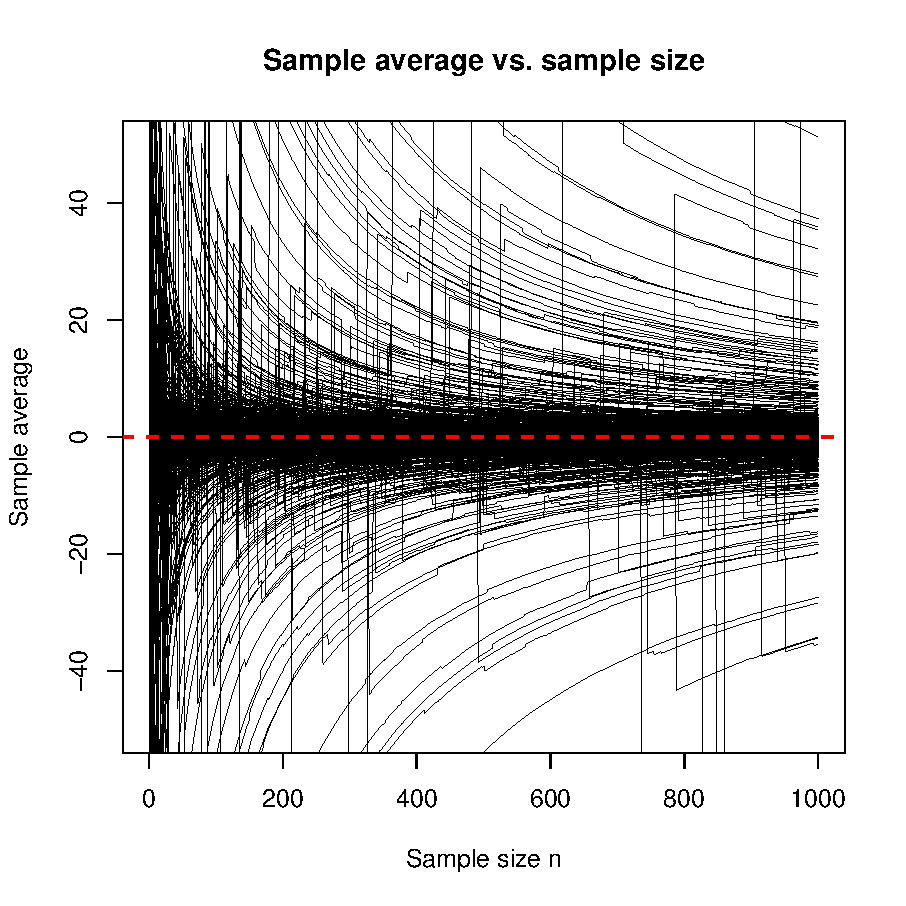
\includegraphics[scale=0.8]{Sample mean of Cauchy.pdf}
    \caption{The 1000 ``sample average $\overline{\xi}_n=\frac{1}{n}\sum_{i=1}^n \xi_i$ vs. sample size $n$" curves.}
    \label{fig: Sample mean of Cauchy}
\end{figure}


%\bibliographystyle{plain}
\bibliography{sample}

\end{document}
